\section{Optimizing Hyperparameter Tuning and AutoML} \label{sec-hyperparam-optimization}
In some workloads, instead of training a model on the data, the user performs a hyperparameter tuning operation.
In the hyperparameter tuning, the user defines a space of possible hyperparameters for the model and train multiple models (sometimes hundreds or thousands) to find the model with the hyperparameters that provides the best performance.
The three common search strategies are grid search, random search, and Bayesian hyperparameter optimization (which is also referred to as the sequential model-based optimization).
In this section, we propose several optimizations to improve the process of hyperparameter tuning.

\subsection{Grid unpacking}
Both grid and random search are a series of individual training operations that only differ in hyperparameters.
To optimize the grid and random search operation, we first transform them into several model training operations through a simple process called grid unpacking.
In grid unpacking, each training operation is considered a separate workload.
Figure \ref{fig-grid-unpacking} shows an example of grid unpacking for a simple SVM Model which has the two hyperparameters penalty (C) and learning rate.
After unpacking, the reuse optimizations techniques discussed in Section \ref{sec-materializaiton-and-reuse} can be applied.
\begin{figure}
\centering
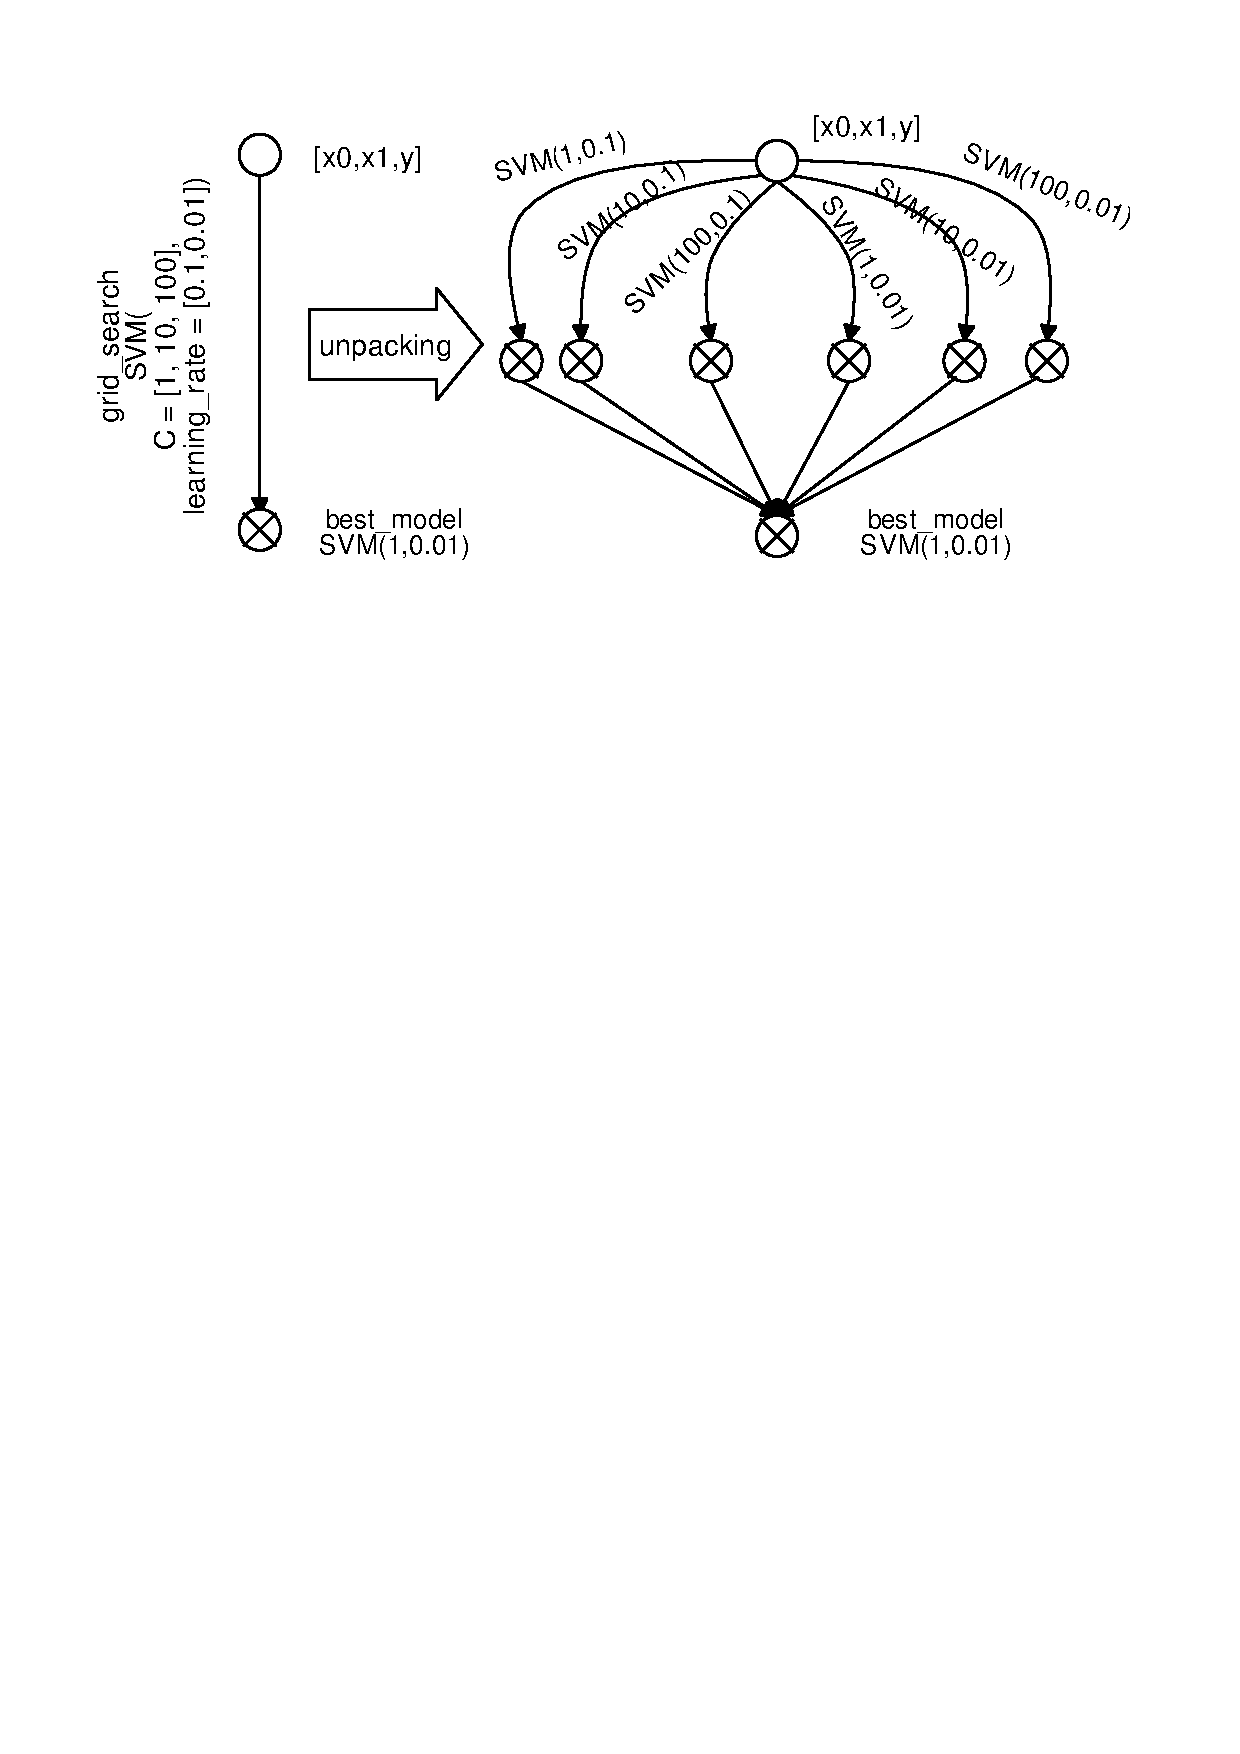
\includegraphics[width=\columnwidth]{../images/grid-unpacking}
\caption{Result of unpacking on a small grid for SVM model. The hyperparameters are C=[1, 10, 100] and learning rate=[0.1, 0.01]}
\label{fig-grid-unpacking}
\end{figure}

\subsection{Automatic Search Space Definition}\label{sub-section-automatic-search-definition}
A major challenge in hyperparameter tuning is defining the search space.
Currently, there is no formal process and typically the search space is defined through experience and common sense.
While this is a less critical issue for expert data scientists, many users struggle with defining the proper range for every hyperparameters before executing the tuning operation.

Extracting the parameter ranges from the experiment database can give us an estimate for defining the search space over undefined hyperparameters, thus, making the search process easier for users that do not have in-depth knowledge of machine learning.
We devise an adaptive strategy to define search space for hyperparameters by utilizing the information in the experiment database.
By utilizing the experiment graph, every existing hyperparameter is mapped to one or several models.
We use the performance of the model (quality metric) to specify a goodness measure for the value of the hyperparameter.
This in turn helps us decide what are the promising and unpromising regions for every hyperparameter in the database.
\todo[inline]{If we end up including AutoML as well, we should mention again that hyperparameters are not just limited to models anymore and any pipeline design decision counts as a (possible) hyperparameter}

\subsubsection{Explorer unit}
One problem when defining the search space having few instances for some specific hyperparameters.
To address this issue, we design a component called the explorer unit.
After a workload is executed, we first determine if there are similar workloads in the experiment database.
Similar workloads are defined workloads that operate on the same dataset.
In case the number of the similar workloads is below a threshold, we invoke the explorer unit to automatically propose values for hyperparameters and find performance of the model trained using each hyperparameter setting.
\todo[inline]{This can be defined as a combination of the existing 'best-practices' and a random walk}

\subsection{Warm Starting the Bayesian Optimization and AutoML}
In this section, we discuss how we use the experiment database to warm start the search process of AutoML and the Bayesian optimization.
Thus, reducing the search time and increasing the probability of finding promising hyperparameter settings faster.
For every existing dataset in the experiment database, we have a corresponding Bayesian optimization process.
We then warmstart the Bayesian optimization process with the existing data transformations, machine learning models, and hyperparameters.

For every new workload, we perform the following.
First, we transform the workload into its graph representation.
Then, we find the corresponding Bayesian optimization process for the dataset in the workload.
Depending on the workload requirement, we perform one of the followings.
\begin{itemize}
\item if the user wishes to find a machine learning pipeline with a specific quality, we resume the Bayesian optimization process until the requirement is met or terminate after a system-defined maximum number of tries ($MAX\_ATTEMPS$).
\item If the user specifies a time budget $MAX\_TIME$, we resume the Bayesian optimization process until the budget is exhausted and return the best (or top $k$) pipeline.
\item If the user requires a pipeline with no quality guarantee and time budget, we return the best existing pipeline back to the user.
\item If no matching Bayesian optimization for the workload exists, we inform the user that automatic optimization is not possible.
\end{itemize}

\subsubsection{Avoiding Local Optima}
Warm starting for hyperparameter optimization and AutoML have the benefit of reducing the overhead of computing many trials.
However, inserting the data from the experiment database into the optimization process may lead the search into local optima.
This could decrease the chance of finding the best hyperparameter setting.
However, our automatic search space definition mechanism alleviates this problem as it explores the regions beyond what is currently defined in the experiment database.
Furthermore, we propose a simple \textit{adaptive warmstarting} method that chooses promising points.
\todo[inline]{Formula for selecting points for warmstarting. It is based on a combination of the quality, how close are points together in the search space, and randomeness}




